\chapter{Results and Analysis}

This chapter presents the results of our timing characterization experiments described in the Chapter 4.
The analysis for these experiments are presented together with the results.
We then present the evaluation for the our mitigation methods presented in Chapter 5.

\section{Impact of data payload size and sampling rate on the overall latency}
The section introduces the results for our experiment 1 described in the \ref{exp1} . 
We use this experiment to analyze the impact of network parameters such as latency and data payload size on the latency.
Since we run this experiment on both the host computers the result will give us indications on the impact of processing resources.\\

Figure \ref{e1_m1} and \ref{e1_m2} shows the results of Experiment 1 for the laptop and desktop computer respectively.
We chose bar graph for visualization of the results as it helps depict the impact of both the data payload size and sampling rate on the overall mean and standard deviation of latency clearly.
The height of each bar represents the mean latency with the standard deviation shown as the error bars on top of each bar.
The latency variation with respect to the data payload size is shown as adjacent bars of different colors.
In these figures, the x-axis shows the sampling rate, the y-axis shows time in $\mu s$.\\

\begin{figure}[h!]
\centering
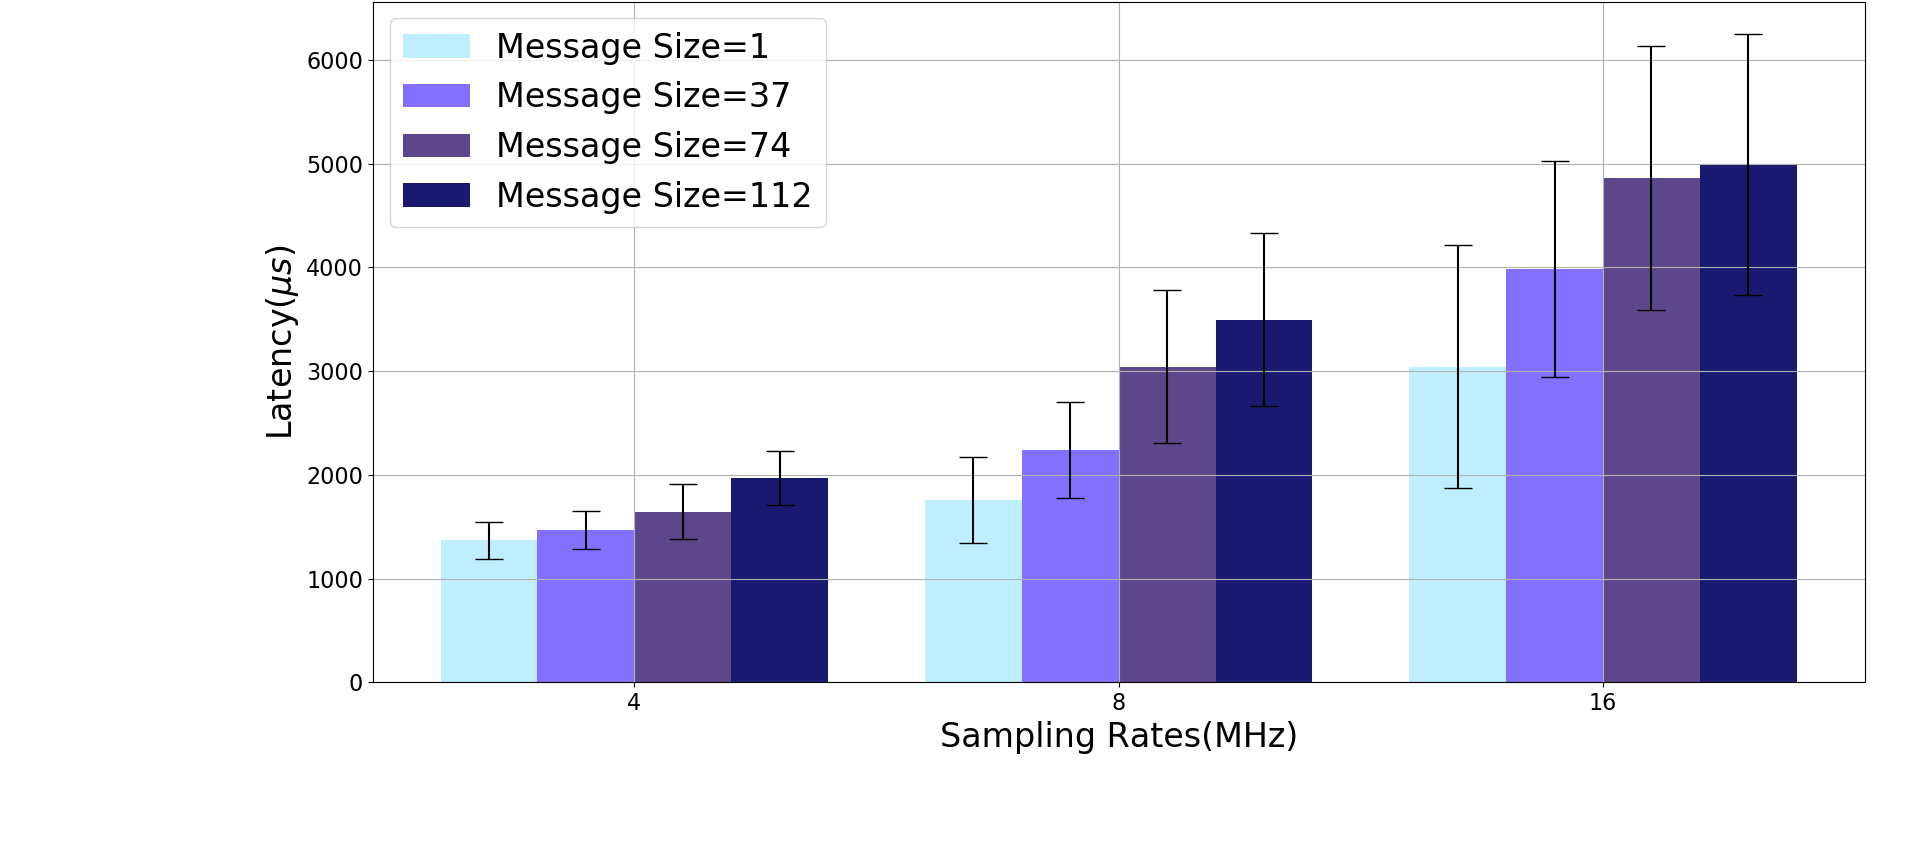
\includegraphics[width=0.8\textwidth]{Thesis/Figure/E1_M1.png}
\caption{Experiment 1: Latency vs Sampling Rates, Message Sizes for laptop(lower processing resources)}
\label{e1_m1}
\end{figure}

\begin{figure}[h!]
\centering
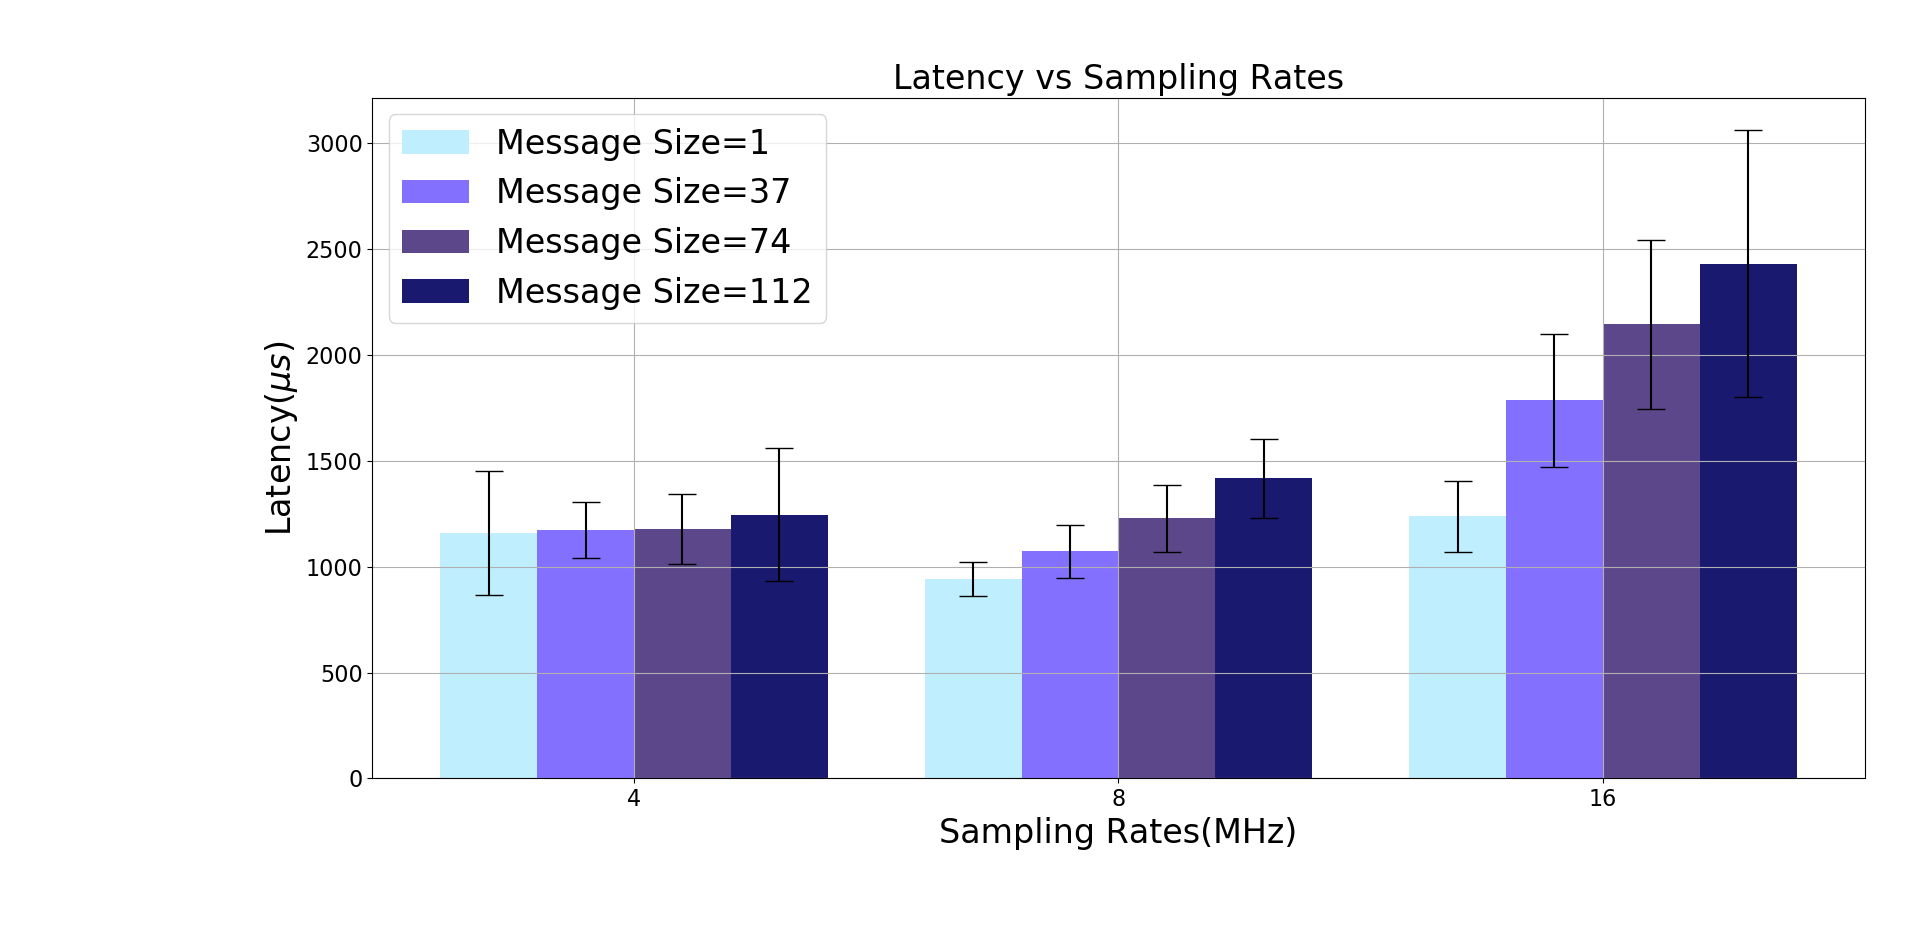
\includegraphics[width=0.8\textwidth]{Thesis/Figure/E1_M2.png}
\caption{Experiment 1: Latency vs Sampling Rates, Message Sizes for desktop(higher processing resources)}
\label{e1_m2}
\end{figure}


The laptop with the lower processing resources shows the the latency increases with increasing sampling rate and increasing data payload size, with message size of one byte for 4 Mhz sampling rate provides the the lowest mean and standard deviation of latency.
The laptop struggles processing the continuous data stream leading to significantly higher mean and standard as shown by the increase in height of the bars and the length of the error bars respectively.
Figure \ref{e1_m1} also highlights the broader trend of higher sampling rates and larger message sizes having higher standard deviation in the latency measurements with all the measurements for 16MHz having standard deviation over 1 ms.
This gives us an indication that we need higher processing resources in order to handle protocols with higher bandwidth requirement.\\

The desktop computer with higher processing resources shows more consistent results for the 4 MHz sampling rate case for all  message sizes.
This is mainly because our definition of latency is asymmetric, making it independent of the data payload size.
For lower message sizes, sampling rate of 8 MHz shows the best results, while diverging with increased data payload size.
The standard deviation of latency for 8 MHz and 16 MHz sampling rate, increases with increase of data payload size, indicating we might need better processing resources for handling the higher bandwidth protocols.
% The measurements for 16 MHz sampling rate for all message sizes struggles, successfully receiving roughly 25 \% of all the messages sent.
% Even those captured latency measurements have high mean and jitter.
Comparison of Figure \ref{e1_m1} and \ref{e1_m2} clearly highlight the impact of processing resources on the latency, with the desktop computer having lower latency for all combinations of the input parameters.\\

% \begin{table}[]
%     \centering
%     \begin{tabular}{|c||c|c|c|}
% \hline
% \backslashbox{Message Sizes}{Sampling Rates} &  4 MHz & 8 MHz & 16 MHz\\
% \hline
%  1 & 290.68 &  79.60 & 167.98 \\
%  37 & 131.32 & 125.30 & 314.63 \\
%  74 &164.07 & 158.25 & 398.92 \\
%  112 & 314.74 & 186.32 & 630.47 \\
% \hline
% \end{tabular}
% \caption{Experiment 1: Standard Deviation(in $\mu s$) of latency measurements for the desktop computer}
%     \label{e1_m2_1}
% \end{table}

% \begin{table}[]
%     \centering
%     \begin{tabular}{|c||c|c|c|}
% \hline
% \backslashbox{Message Sizes}{Sampling Rates} &  4 MHz & 8 MHz & 16 MHz\\
% \hline
% 1 & 179.10 & 414.97 & 1174.68 \\
% 37 &  182.97 & 460.83 & 1042.72 \\
% 74 & 261.39 & 737.14 & 1273.21 \\
% 112 & 262.88 & 835.26 & 1257.05 \\

% \hline
% \end{tabular}
% \caption{Experiment 1: Standard Deviation(in $\mu s$) of latency measurements for the laptop}
%     \label{e1_m1_1}
% \end{table}


\section{Component Delay Analysis}
In this section, we present the results of the Experiment 2 described in \ref{exp2}.
We analyze the results of this experiment to get a deeper understanding of the system and investigate the reasons for the results shown in the previous section.
This results and subsequent analysis also helps us in the selection of our mitigation strategies.\\

\begin{figure}[h!]
\centering
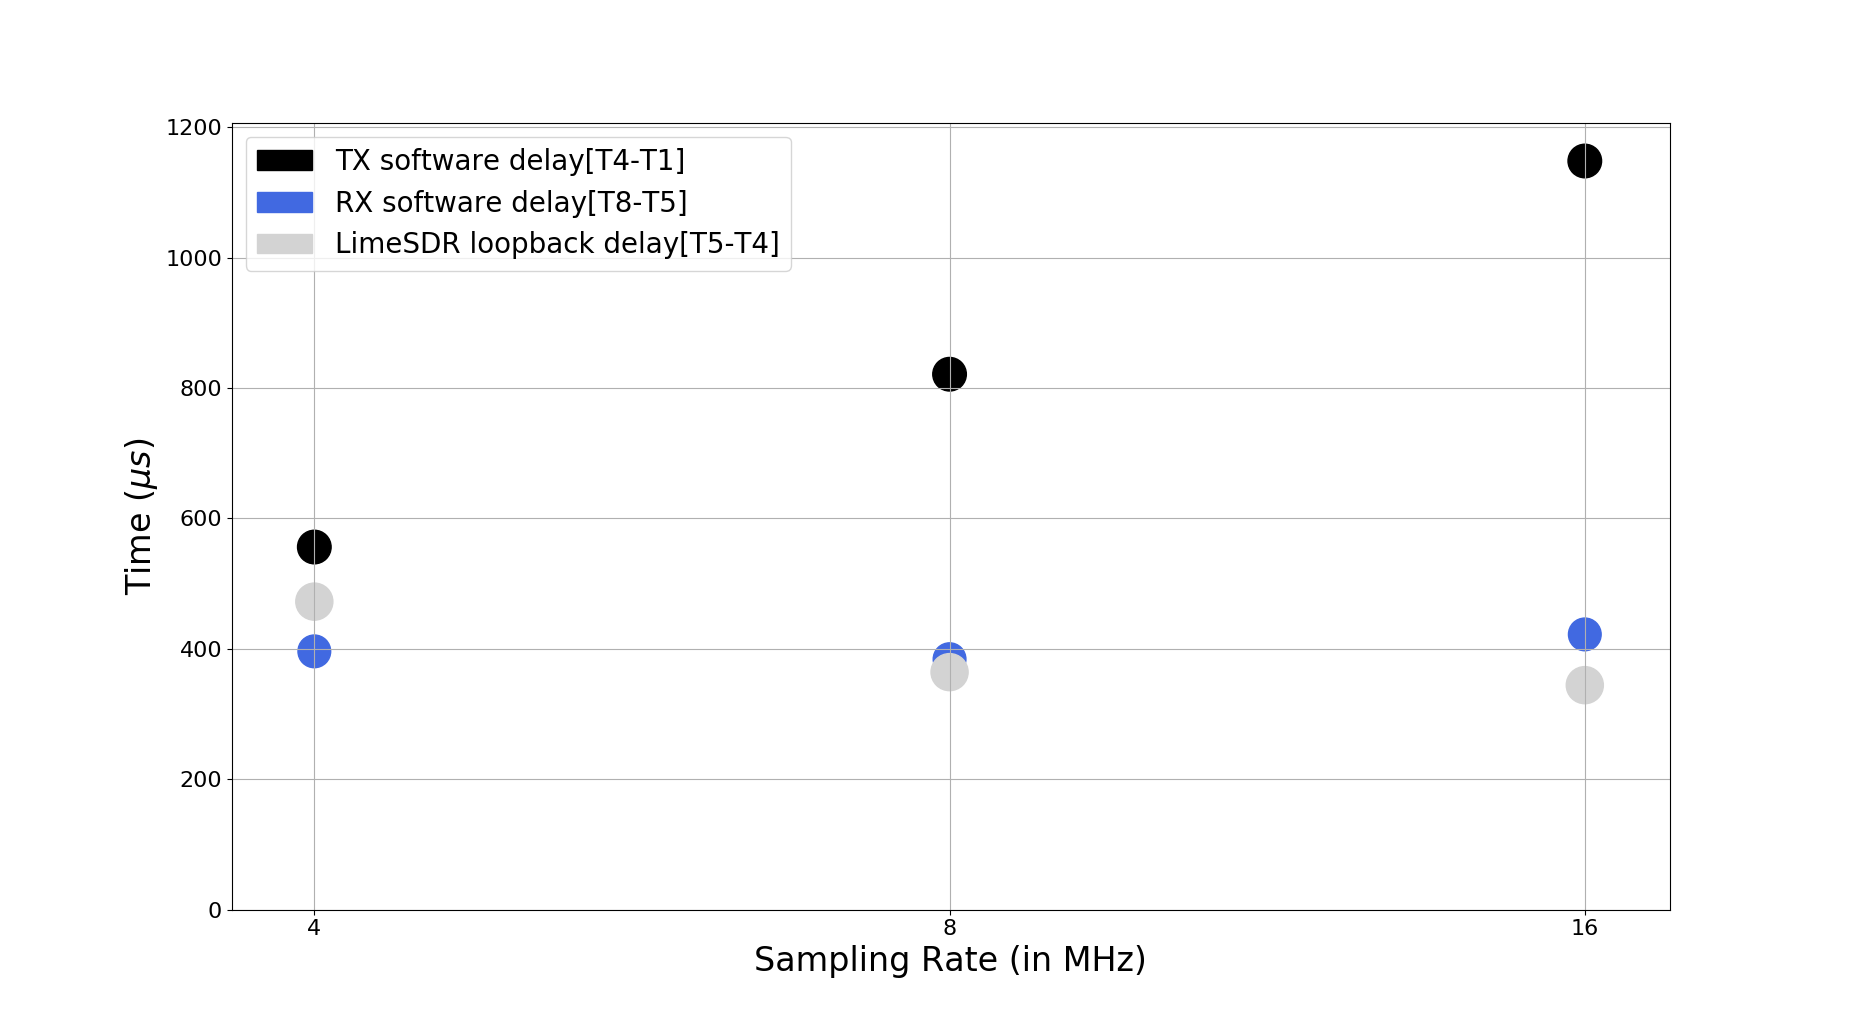
\includegraphics[width=0.8\textwidth]{Thesis/Figure/E2_M1.png}
\caption{Experiment 2: Component Delays vs Message Sizes for laptop(lower processing resources)}
\label{e2_m1}
\end{figure}

\begin{figure}[h!]
\centering
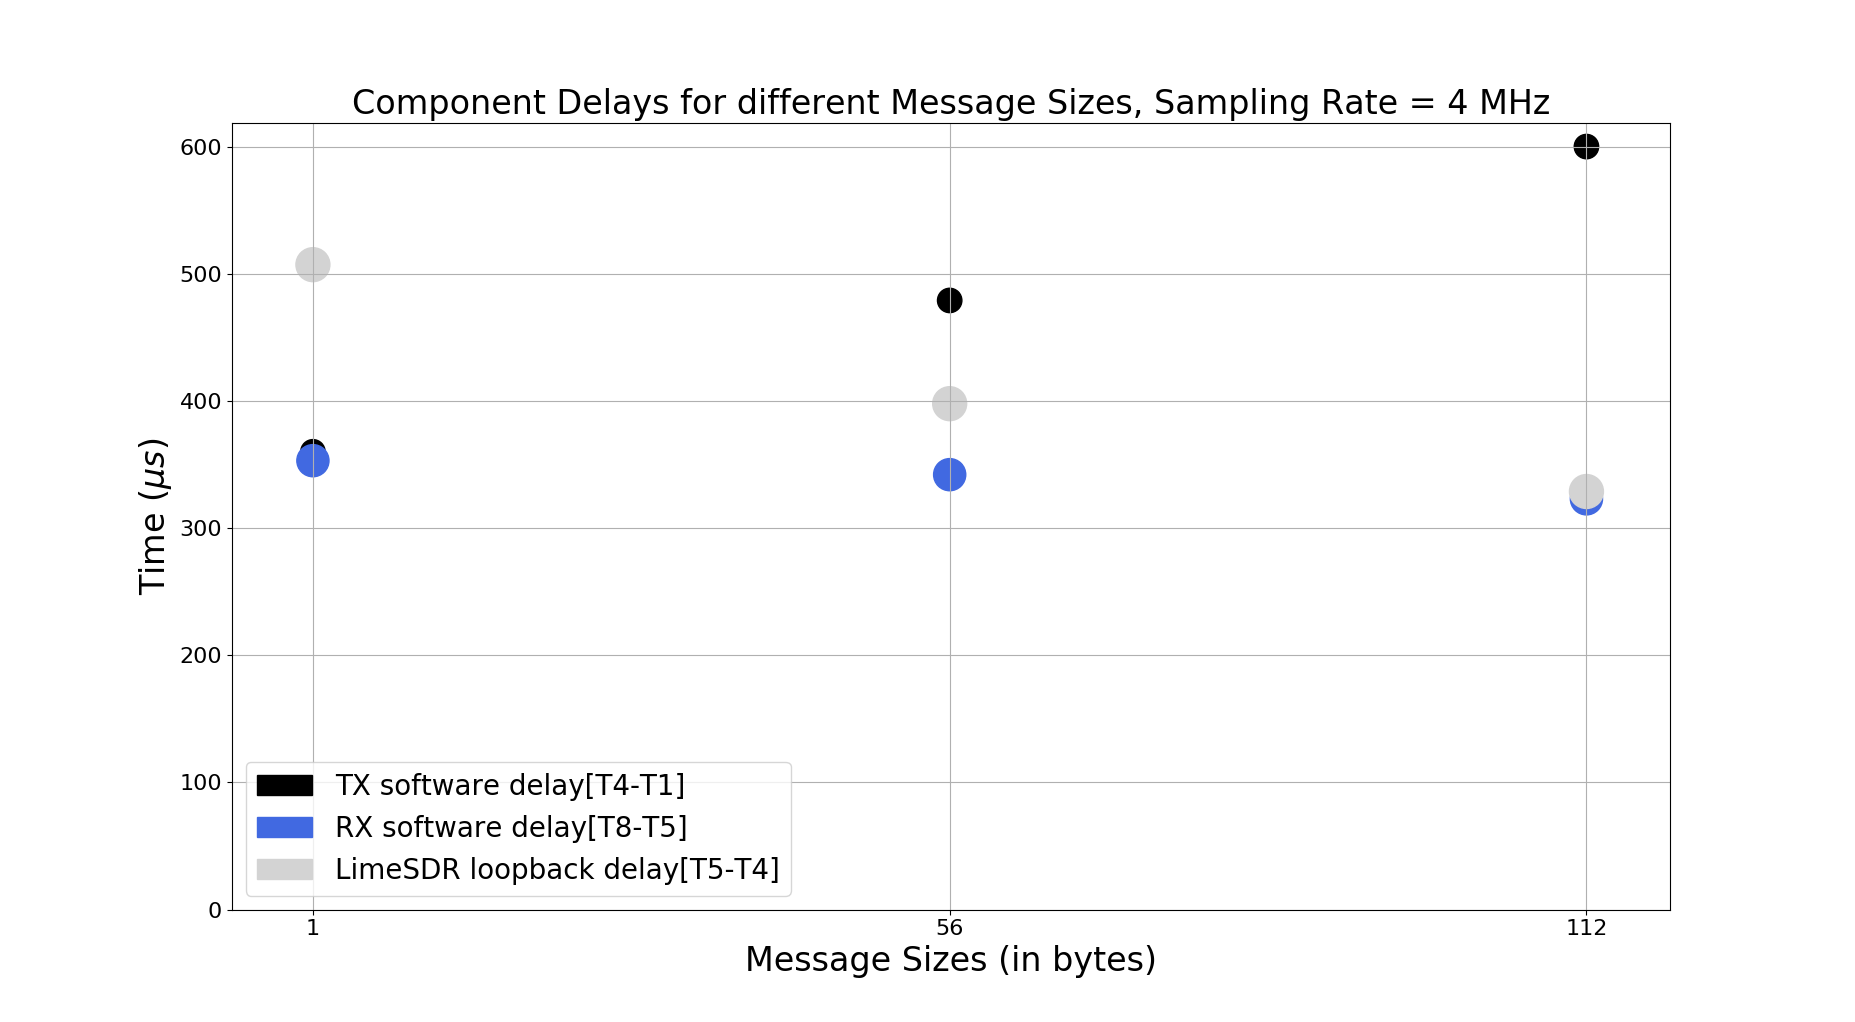
\includegraphics[width=0.8\textwidth]{Thesis/Figure/E2_M2_1.png}
\caption{Experiment 2: Component Delays vs Message Sizes for desktop(higher processing resources)}
\label{e2_m2}
\end{figure}


Figure \ref{e2_m1} and \ref{e2_m2} shows the results of the component delays  for the laptop and desktop respectively.
The x-axis shows the data payload size and the y-axis shows the component delays in $\mu s$.
The results have been shown using bubble plot as it helps understand both the median of the data samples and variation of the measurements.
The height of each bubble shows the median delay whereas the area of the bubbles show the difference in latency between the 95 percentile value and the 5 percentile value.
This helps us visualize the variation of component delays across measurement data samples.
The larger the area of the bubble, higher the amount of jitter contributed by it.\\

Both the results show an increase in TX software delays ($T_4 - T_1$) with message sizes.
This is understandable as the TX software chain needs to process more data for higher data payload size.
Although the rate of increase is different for both the computers, with the laptop measurements showing a faster rate of increase compared to the desktop computer.
The GNU Radio TX flowgraph is processing intensive, the higher CPU clock speed and higher number of CPU cores helps the desktop computer to desktop computer to process faster.
The RX software delay ($T_8 - T_5$) is more or less constant across the message sizes.
It is primarily because of our definition of $T_8$, the RX software chain needs to process the same amount of data regardless of the data payload size.
The desktop computer performs slightly better compared to the desktop computer, taking approximately (insert value) less time.\\

The LimeSDR loopback delay ($T_5 - T_4$) decreases with message sizes.
We hypothesize this pattern is caused by the the buffering of data between the LimeSDR \ac{FPGA} and Cypress EZ-FX3 on the TX Path of the LimeSDR-USB.
So lower amount of data needs to shift across these buffers before finally reaching the \ac{FPGA} TX Path for transmission.
The shift clock for the TX FIFOs is dependent on the sampling rate, which is 4MHz while the buffer write clock is 100 MHz.
For larger message sizes, the buffer is filled up faster as more data is available hence it needs to shift for significantly shorter time. \\

The measurements across both the computers have similar LimeSDR loopback delays, indicating that our time probes placement for the measurement are correct and the measurements are independent of the host computer processing resources.
Our uniform results across message sizes for 4MHz sampling rate (shown in Figure \ref{e1_m2}) for the desktop computer can be attributed to compensation of the increase of TX processing delay by the decrease LimeSDR loopback delay.
In case of the laptop, although the LimeSDR loopback delay decreases, the TX processing time increases faster with increase in message sizes.
Hence, the total latency increases with data payload size as the RX software chain delay is more or less constant.

\begin{figure}[h!]
\centering
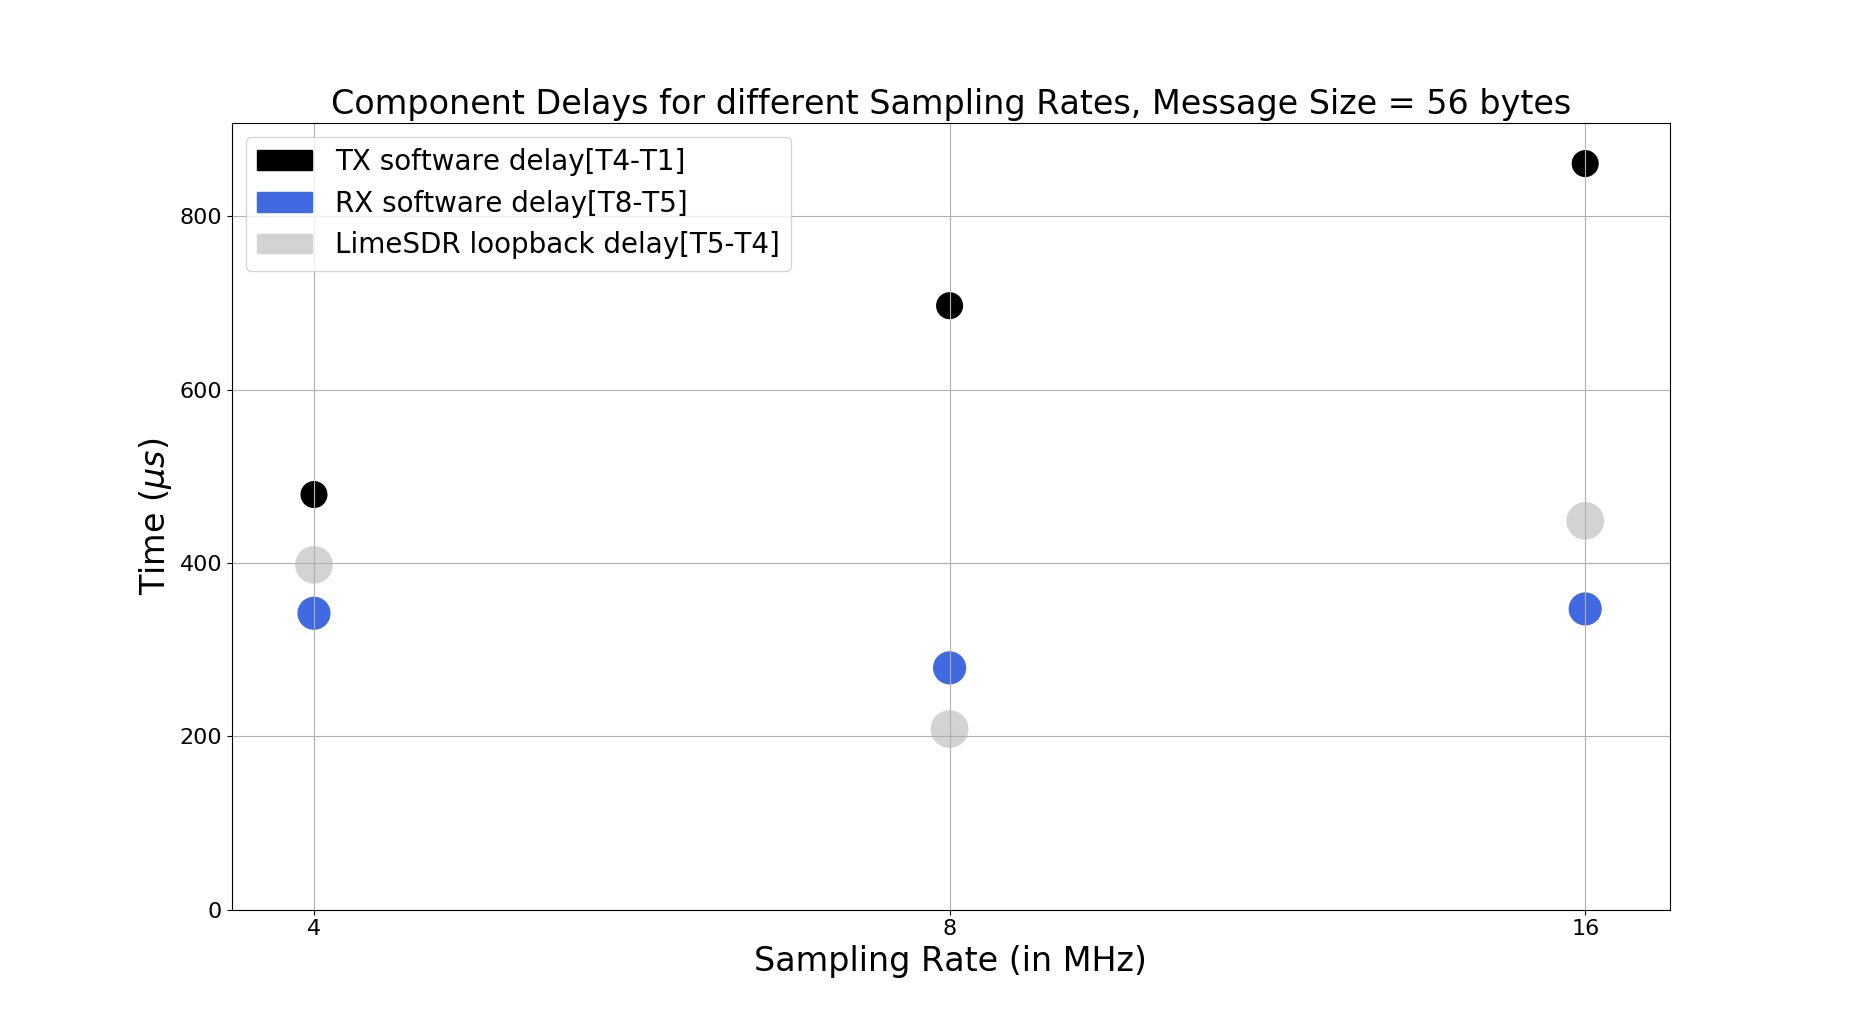
\includegraphics[width=0.8\textwidth]{Thesis/Figure/E2_M2_2.png}
\caption{Experiment 2: Component Delays vs Sampling Rates for the desktop computer(higher processing resources)}
\label{e2_m2_1}
\end{figure}

An additional experiment was performed on the desktop computer for measuring the impact of sampling rate on component delays.
The LimeSDR loopback delay decreases for the 8 MHz sampling rate, the measurement for 16 MHz increases because we had to increase the USB transfer size to have reasonable amount of measurement samples.
The decrease of LimeSDR loopback delay with sampling rate explains the decrease of overall latency for sampling rate of 8 MHz, shown in Figure \ref{e1_m2}.
The TX software chain delay increases with sampling rate as it has to process more data samples.

\section{Impact of USB Transfer size} \label{ex3:results}
This section presents the results for Experiment 3 which was described in \ref{exp3}.
The results help us analyzing the impact of batchsize of LimeSDR FPGA packet size on the overall latency and how component delays are affected by the increase in the USB Transfer size.
These results further provide us the motivation for our mitigation strategy.\\

\begin{figure}[h!]
\centering
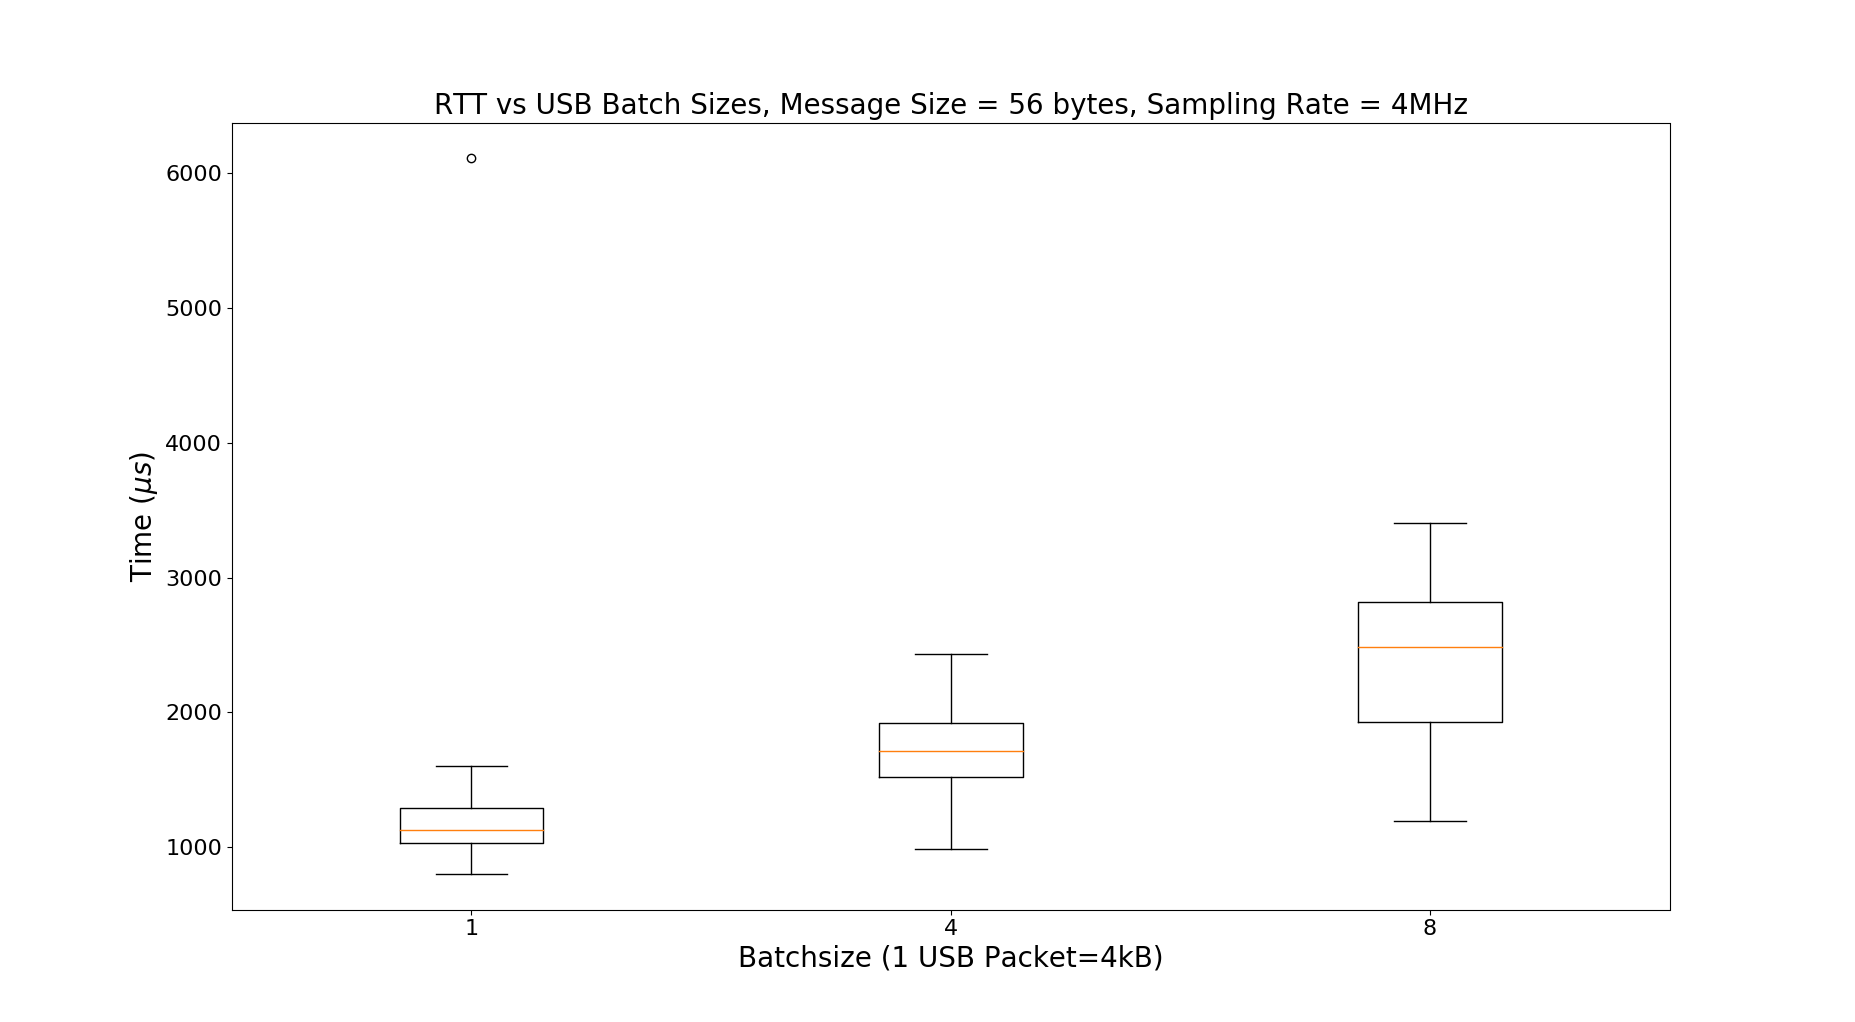
\includegraphics[width=0.8\textwidth]{Thesis/Figure/E3M2-1.png}
\caption{Experiment 3: Mean Latency vs Batchsize of LimeSDR FPGA packets (1 FPGA packet = 4096 bytes)}
\label{e3_1}
\end{figure}

\begin{figure}[h!]
\centering
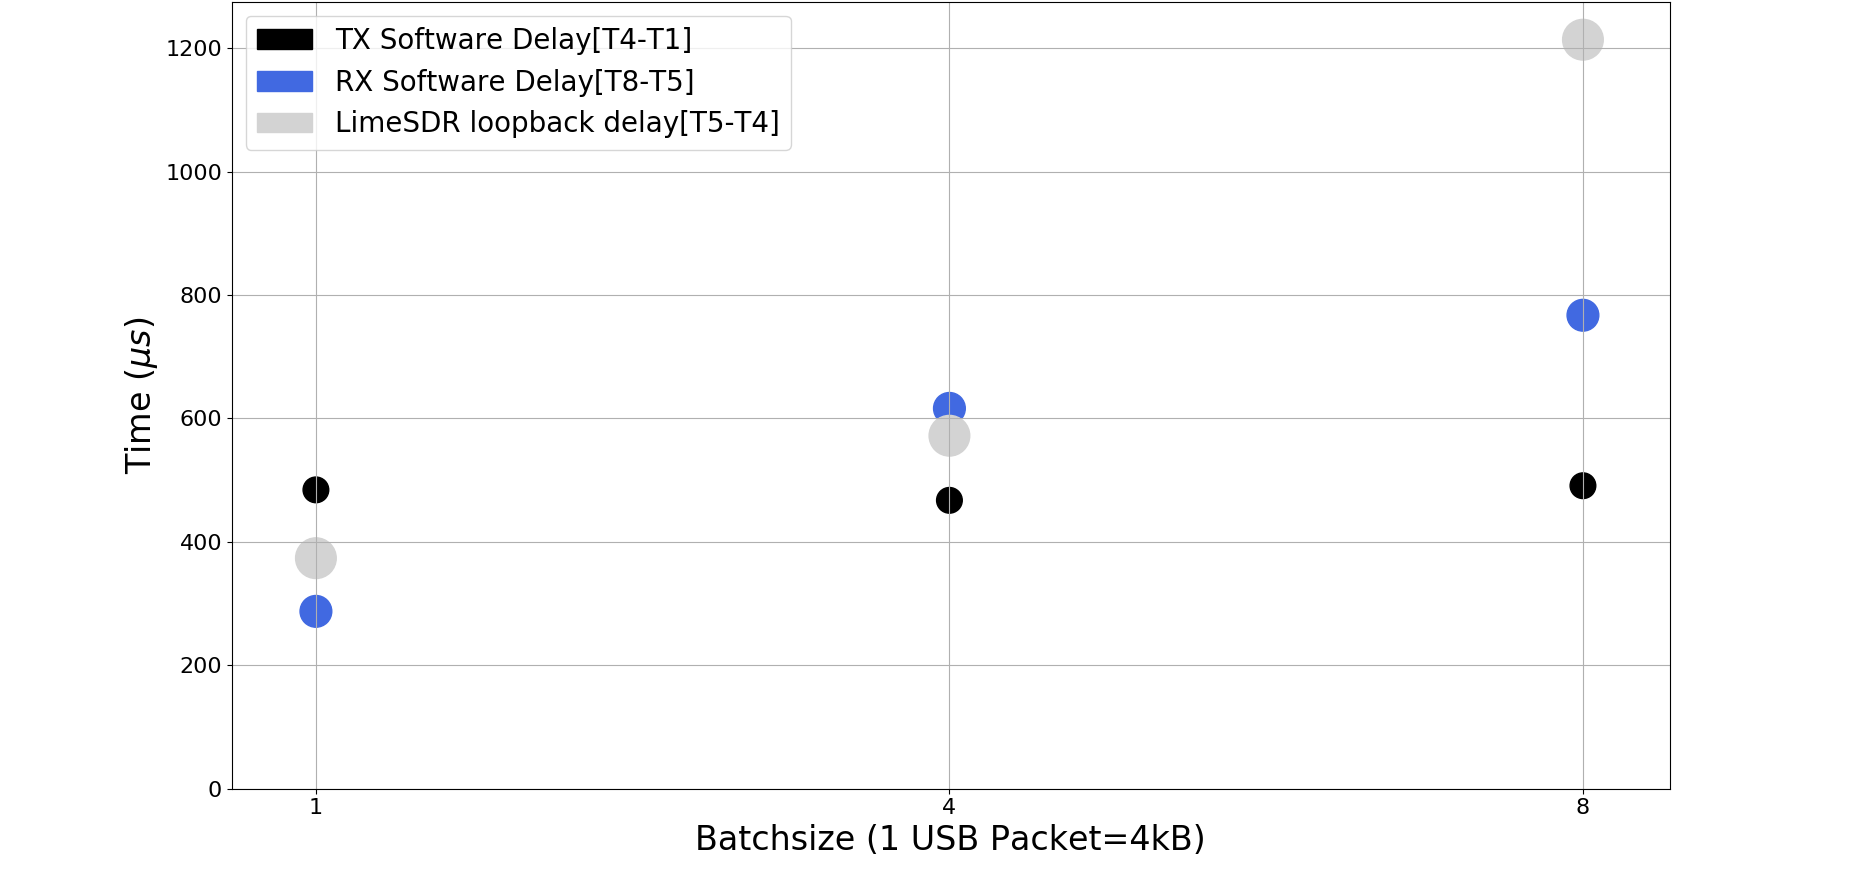
\includegraphics[width=0.8\textwidth]{Thesis/Figure/E3M2-2.png}
\caption{Experiment 2: Component Delays vs Batchsize of LimeSDR FPGA packets}
\label{e3_2}
\end{figure}

Figure \ref{e3_1} shows the box plots for the latency measurements for three different batchsizes: 1,4 and 8. 
The box plots shows that the latency and jitter increases as the batchsize increases.
This results can be analyzed with the help of Figure \ref{e3_2} which shows the component delays for these latency measurements as bubble plots.
The increase of LimeSDR loopback delay contributes significantly to the increase of overall latency and jitter as evident from the increase in height and area of the blue bubbles representing LimeSDR loopback delay in Figure \ref{e3_2}.
This result is consistent with the analysis of Schmid et al \cite{schmid_experimental_2007} that the bus transfer time is dependent on the sampling rates.
It takes  255 $\mu s$ to generate samples for one FPGA Packet with 4 MHz sampling rate, while it takes 1020 $\mu s$ and $2040 \mu s$ respectively to generate samples for four and eight LimeSDR FPGA packets respectively.
For this reason, the LimeSDR loopback delay increases with higher batchsizes.
With 8 MHz sampling rate it takes 127.5 $\mu s$ to generate the samples needed for one FPGA packet, this explains the decrease of LimeSDR loopback delay in Figure \ref{e2_m2_1} for the 8MHz sampling rate measurements.\\

Figure \ref{e3_2} also shows that the LimeSDR loopback delay for batchsize set to one is greater the time needed to generate the samples, while its lower than the sample generation time for batchsize four and eight.
This leads us to believe that the TX Path delays are significant with respect to sample generation time for one FPGA packet.
The RX software chain delays increases slightly with increase of batchsizes, as the GNU Radio blocks now process more data samples in one execution.
The TX software chain delays are constant across all three batchsizes.\\

\section{Evaluation of mitigation strategies}
This section introduces the results for Experiment 4(\ref{exp4}).
The results focuses on the impact of LimeSDR packet size and GNU radio \texttt{max\_noutput\_items} on the overall latency and component delays.
The percentage of CPU usage collected using \texttt{pidstat} is used for analyzing the obtained results with respect to the host computer processing resources.\\

\begin{figure}[h!]
\centering
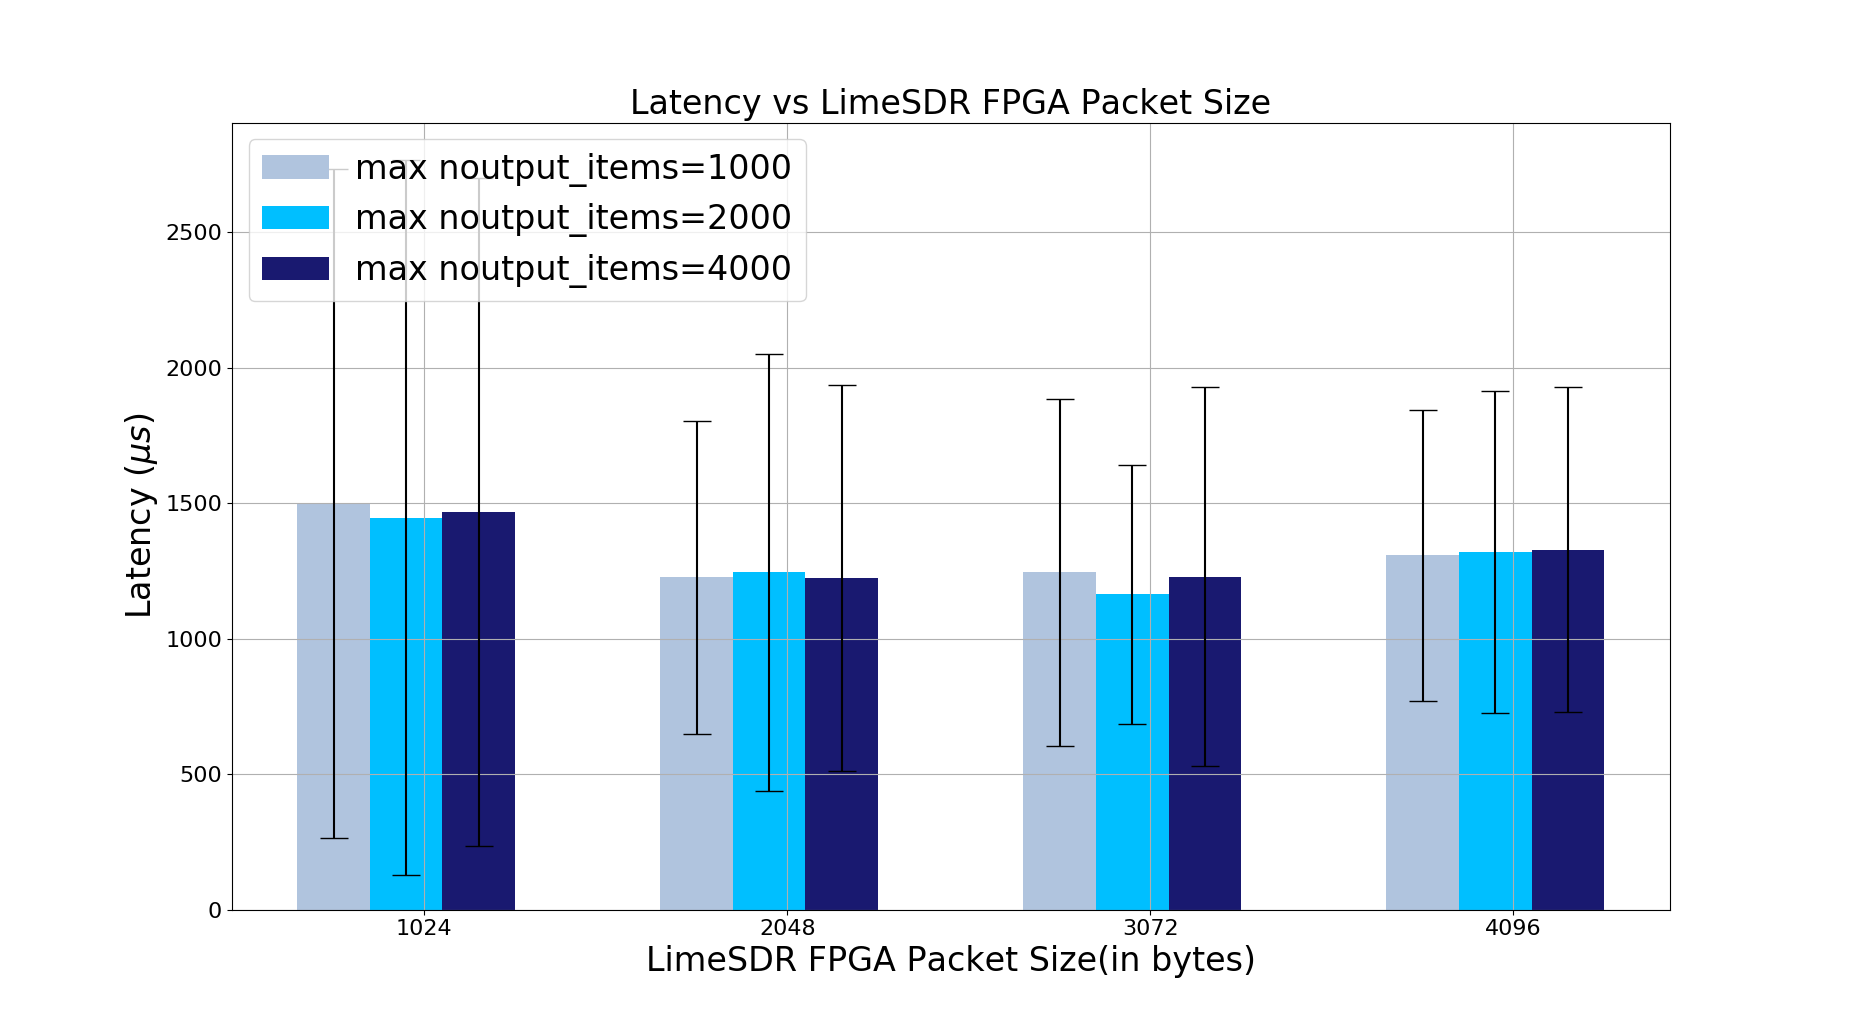
\includegraphics[width=0.8\textwidth]{Thesis/Figure/E4_M1_1.png}
\caption{Experiment 4: Latency vs LimeSDR FPGA packet size for the laptop (lower processing resources)}
\label{e4_m1_1}
\end{figure}

\subsection{Impact on latency}
Figure \ref{e4_m1_1} and \ref{e4_m2_1} shows the results for the laptop and desktop computer respectively.
We use bar graph for visualizing the results as it helps in easier representation of both the mean and standard deviation of our measurements with respect to the input parameters.
The LimeSDR FPGA packet size is represented in bytes along the x-axis, with the y-axis representing the latency ($T_8 - T_1$) in $\mu s$.
The height of each bar represents the mean latency, the standard deviation of the latency is shown as  error bars.
The variation of overall latency with GNU radio \texttt{max\_ noutput\_items} is shown for each LimeSDR FPGA packet size as adjacent bar plots in different shades of blue.\\

We get the lowest mean and standard deviation of latency for LimeSDR FPGA packet size of 3072 bytes with \texttt{max\_noutput\_items} set to 2000 for the laptop.
This configuration of input parameters decreases the mean and standard deviation of latency to  1165 $\mu s$ and 478 $\mu s$  from 1329 $\mu s$ and 599 $\mu s$ for the default configuration of the LimeSDR-USB platform.
Latency for LimeSDR FPGA sizes of 1024 bytes and 2048 bytes shows high mean and standard deviations which is in contrast to our understanding of lower LimeSDR FPGA packet size leads to lower latency because of lower LimeSDR loopback delay. This will be analyzed later with respect to the processing resources.\\

\begin{figure}[h!]
\centering
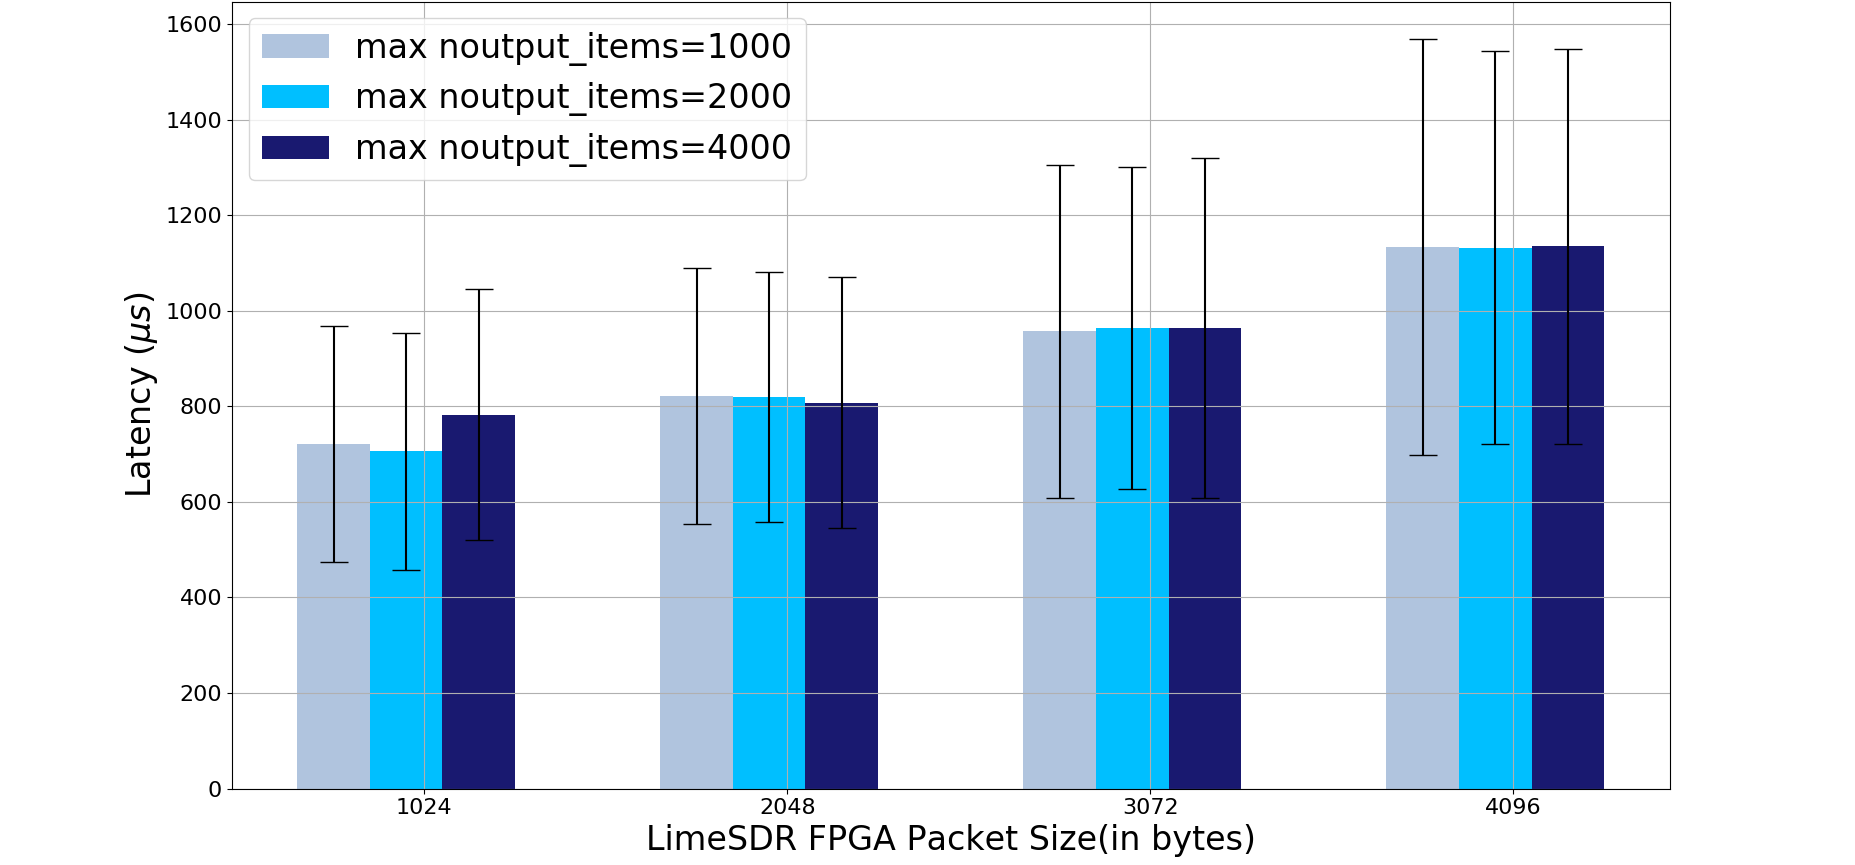
\includegraphics[width=0.8\textwidth]{Thesis/Figure/E4_M2_1.png}
\caption{Experiment 4: Latency vs LimeSDR FPGA packet size for the desktop computer (higher processing resources)}
\label{e4_m2_1}
\end{figure}

The results for the desktop computer shows lower LimeSDR FPGA packet sizes leads to with lower latency with less standard deviation.
We get the lowest latency and jitter for LimeSDR FPGA packet size of 1024 bytes and \texttt{max  n\_out-\\put\_items} set to 2000 data elements.
This combination of input parameters results in mean and standard deviation of latency decreasing to 706 $\mu s$ and 248 $\mu s$ respectively from 1135 $\mu s$ and 414 $\mu s$ for the default configuration.
These results from the desktop computer indicates the results in Figure \ref{e4_m1_1} is definitely impacted by the processing resources of the host computer as the lower LimeSDR FPGA packet sizes results in high mean and standard deviation of latency\\

In both the host computers, the impact of GNU radio \texttt{max\_noutput\_items} is arbitrary across combinations of the input parameters.
Since we didn't pass a strict condition to the GNU radio scheduler and the operation of scheduler is like a black box to us, we can not determine the causal effect of \texttt{max\_noutput\_items} on latency exactly.
We will use component delay analysis to find its impact on the RX and TX Software chains to gain some insight about its impact.\\

\subsection{Impact on the component delays}
\begin{figure}[h!]
\centering
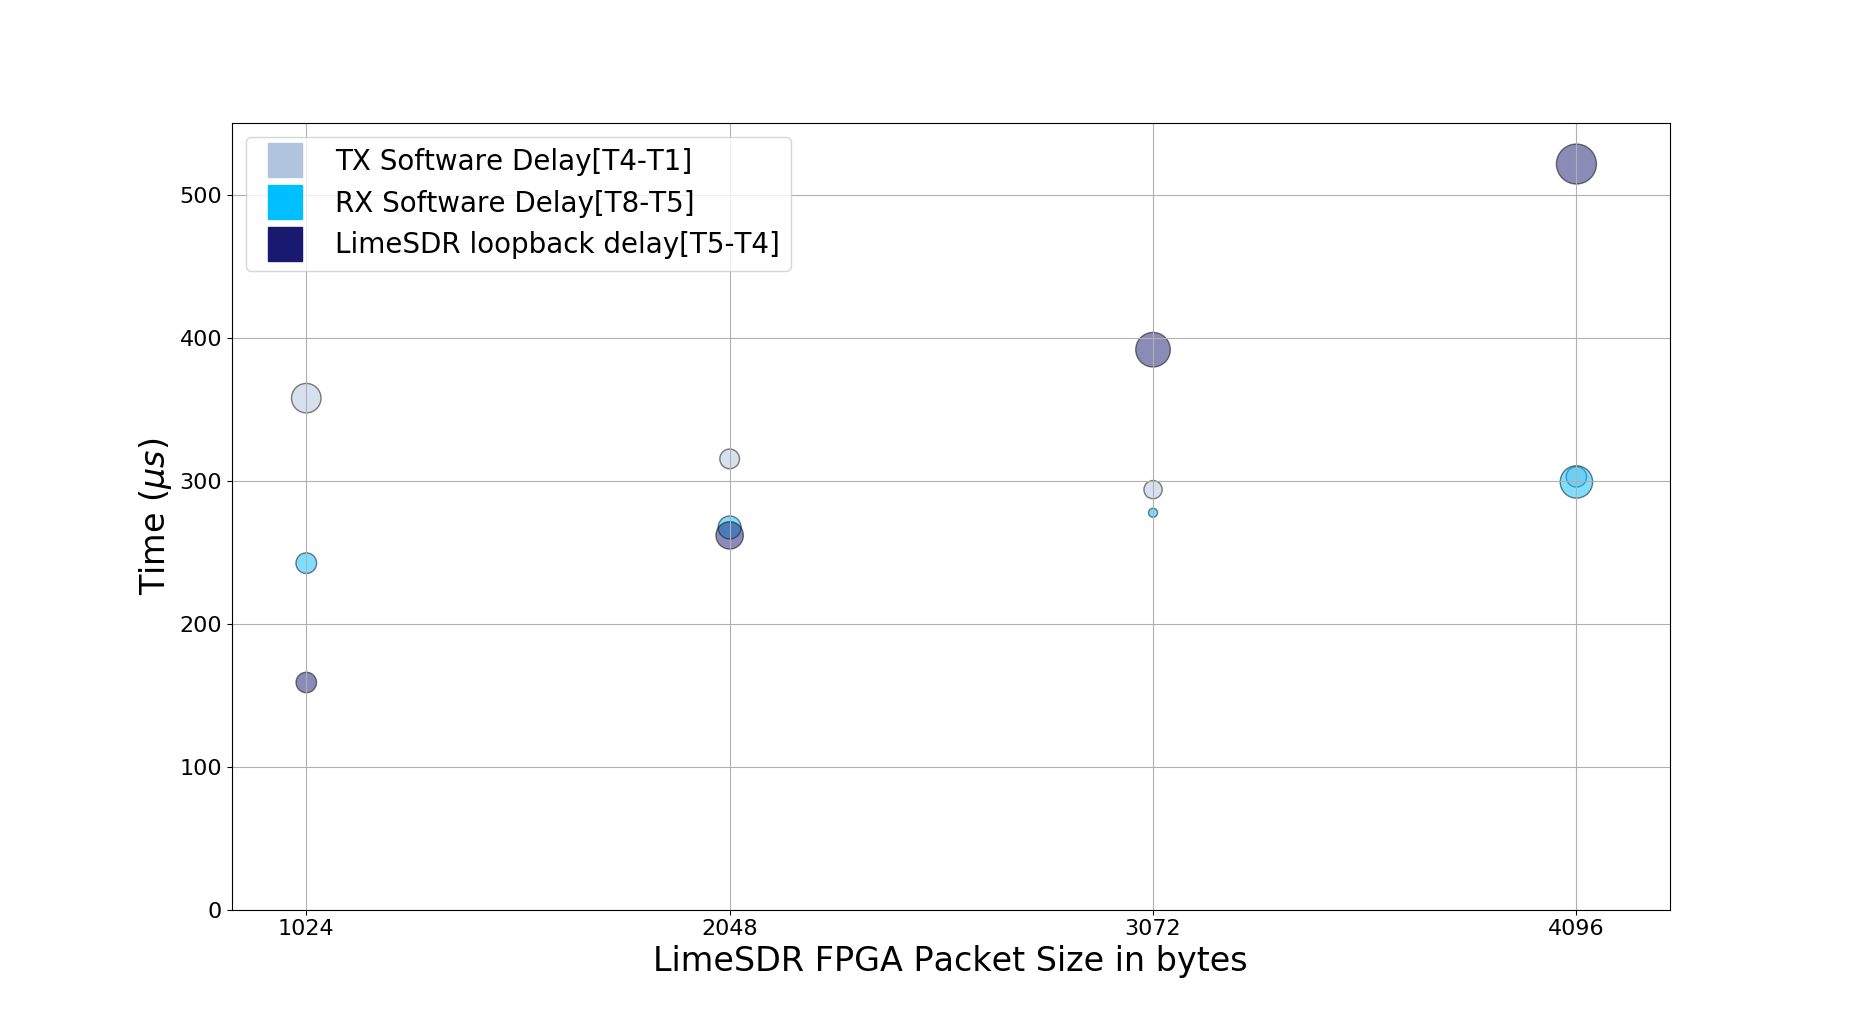
\includegraphics[width=\textwidth]{Thesis/Figure/E4M2-2.png}
\caption{Experiment 4: Component Delays vs LimeSDR FPGA packet size for the desktop computer (higher processing resources)}
\label{e4_m2_2}
\end{figure}

The component delays for different LimeSDR FPGA packet sizes with \texttt{max\_nout-put\_items} set to 2000 on the desktop computer is shown in Figure \ref{e4_m2_2}.
The RX software delays and the TX software delays are further segmented into their individual component delays as shown in Figure \ref{e4_m2_3} and \ref{e4_m2_4} respectively.
The results are shown as a bubble plot, with the height of the marker representing the mean value, while the area of the bubble representing the difference between the $95^{th}$ percentile and $5^{th}$ percentile value of the relevant component delays we have collected.
The LimeSDR FPGA packet size is represented in bytes along the x-axis, with the y-axis representing time in $\mu s$.\\

LimeSDR loopback delay increases as we increase the LimeSDR FPGA packet size as evident from the height of the markers representing the LimeSDR loopback delay.
Increasing LimeSDR FPGA packet size also increases the area of the markers, indicating higher variance of the LimeSDR loopback delay. 
These results follows the trend we estimated using Equation \ref{eq4}, although the quantitative value for each of these measurements are higher than those shown in Table \ref{min-max}, indicating there is additional delays on the TX Path and transfer.
These results are shown for data payload size of 10 bytes and the LimeSDR loopback delay for the the default configuration is same as that shown in Figure \ref{e2_m2} for one byte data payload.
We hypothesized that the LimeSDR loopback delay may be affected by the buffering between the EZ-FX3 and FPGA as the data samples would have to shift through the buffers, this hypothesis also holds for the measurements shown here as we are measuring for lower data payload size.\\

\begin{figure}[h!]
\centering
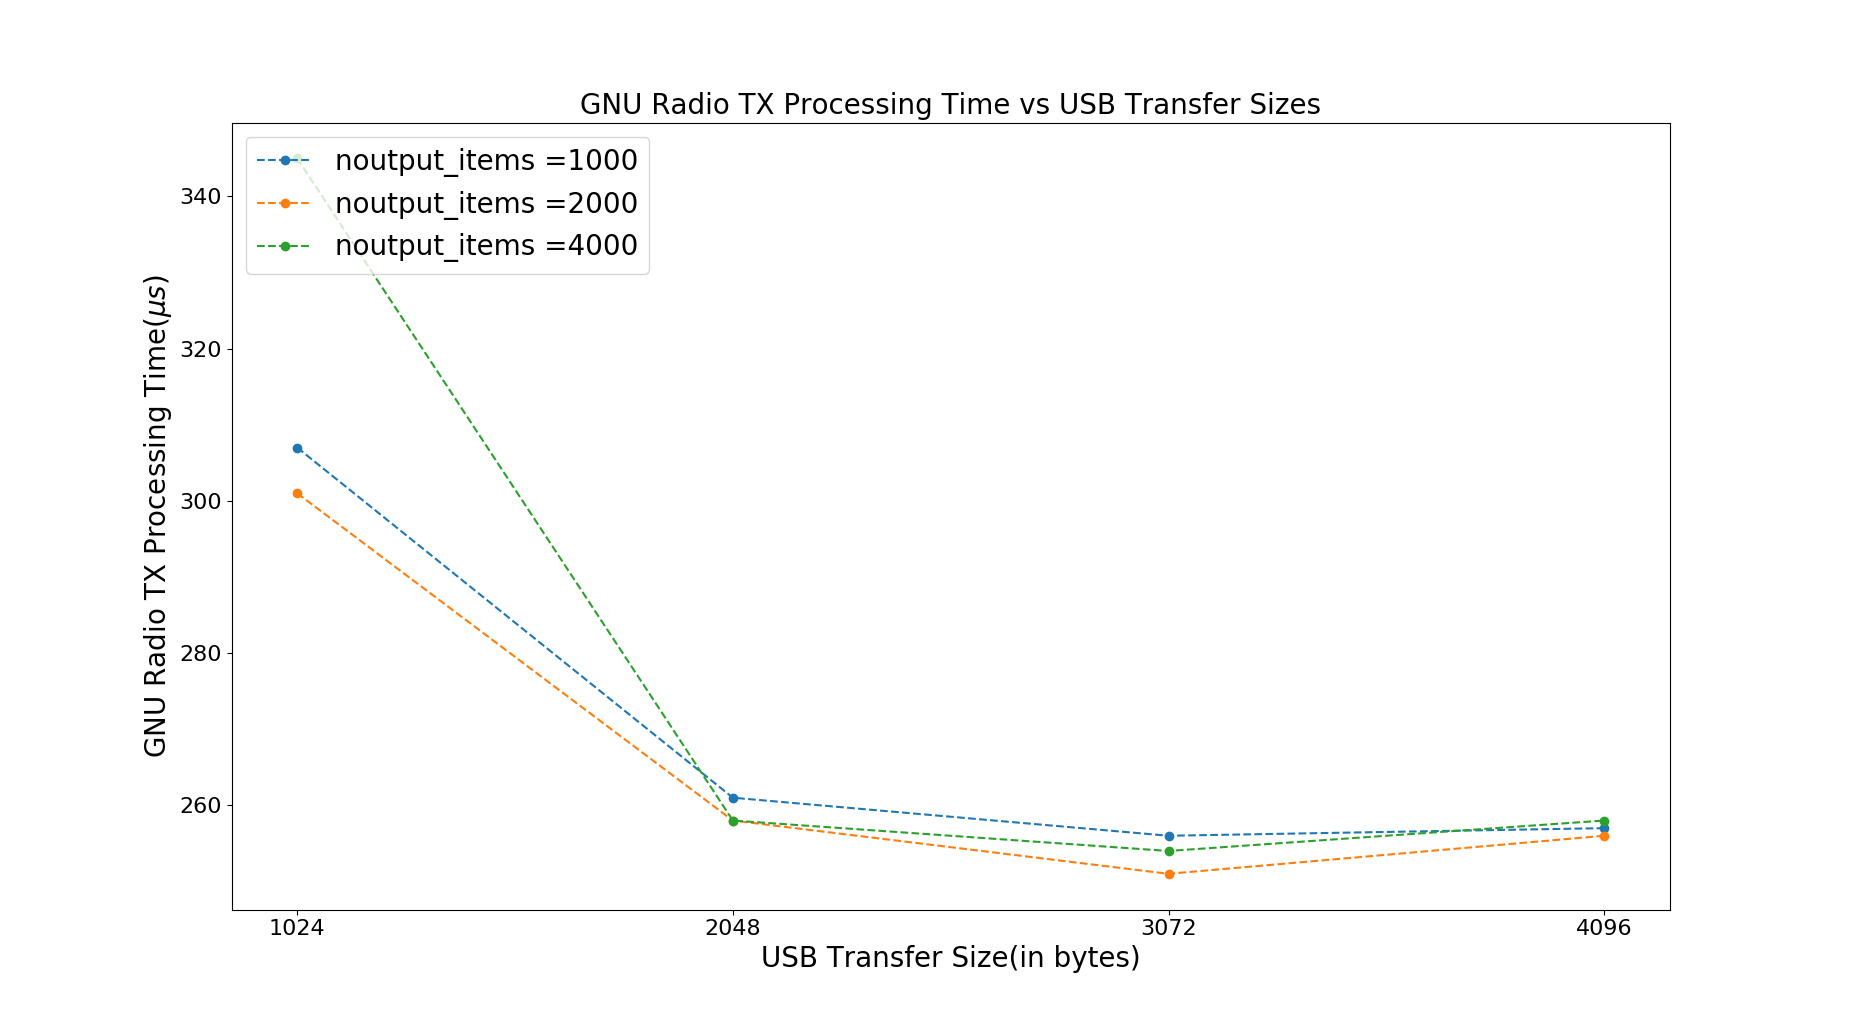
\includegraphics[width=\textwidth]{Thesis/Figure/E4M2-3.png}
\caption{Experiment 4: RX Software Chain Component Delays vs LimeSDR FPGA packet size for the desktop computer (higher processing resources)}
\label{e4_m2_3}
\end{figure}

The RX software chain delay increases slightly with increase in the LimeSDR FPGA packet size as shown in Figure \ref{e4_m2_2}.
As the LimeSDR FPGA packet size increases, the GNU Radio scheduler will allocate the blocks to process higher number of data elements to process in one execution, which results in slightly increased GNU Radio processing time as shown by the trend shown in Figure \ref{e4_m2_3}.
We see that the kernel to user space delay decreases slightly as we increase the LimeSDR FPGA packet size.
This slight increase for lower LimeSDR FPGA packet sizes can be attributed to increase of USB driver system calls.\\

We observed that the \texttt{max\_noutput\_items} parameter doesn't impact both the RX software delay and the LimeSDR delay.
LimeSDR loopback delay is independent of the GNU Radio run time configuration, hence it is not affected by the \texttt{max\_noutput\_items} parameter.
For the RX software chain, the results can be interpreted as either there is no GNU Radio block which has higher processing delays to be affected by the \texttt{max\_noutput\_items} parameter or the decrease in processing delay is compensated by the increased signalling.\\

\begin{figure}[h!]
\centering
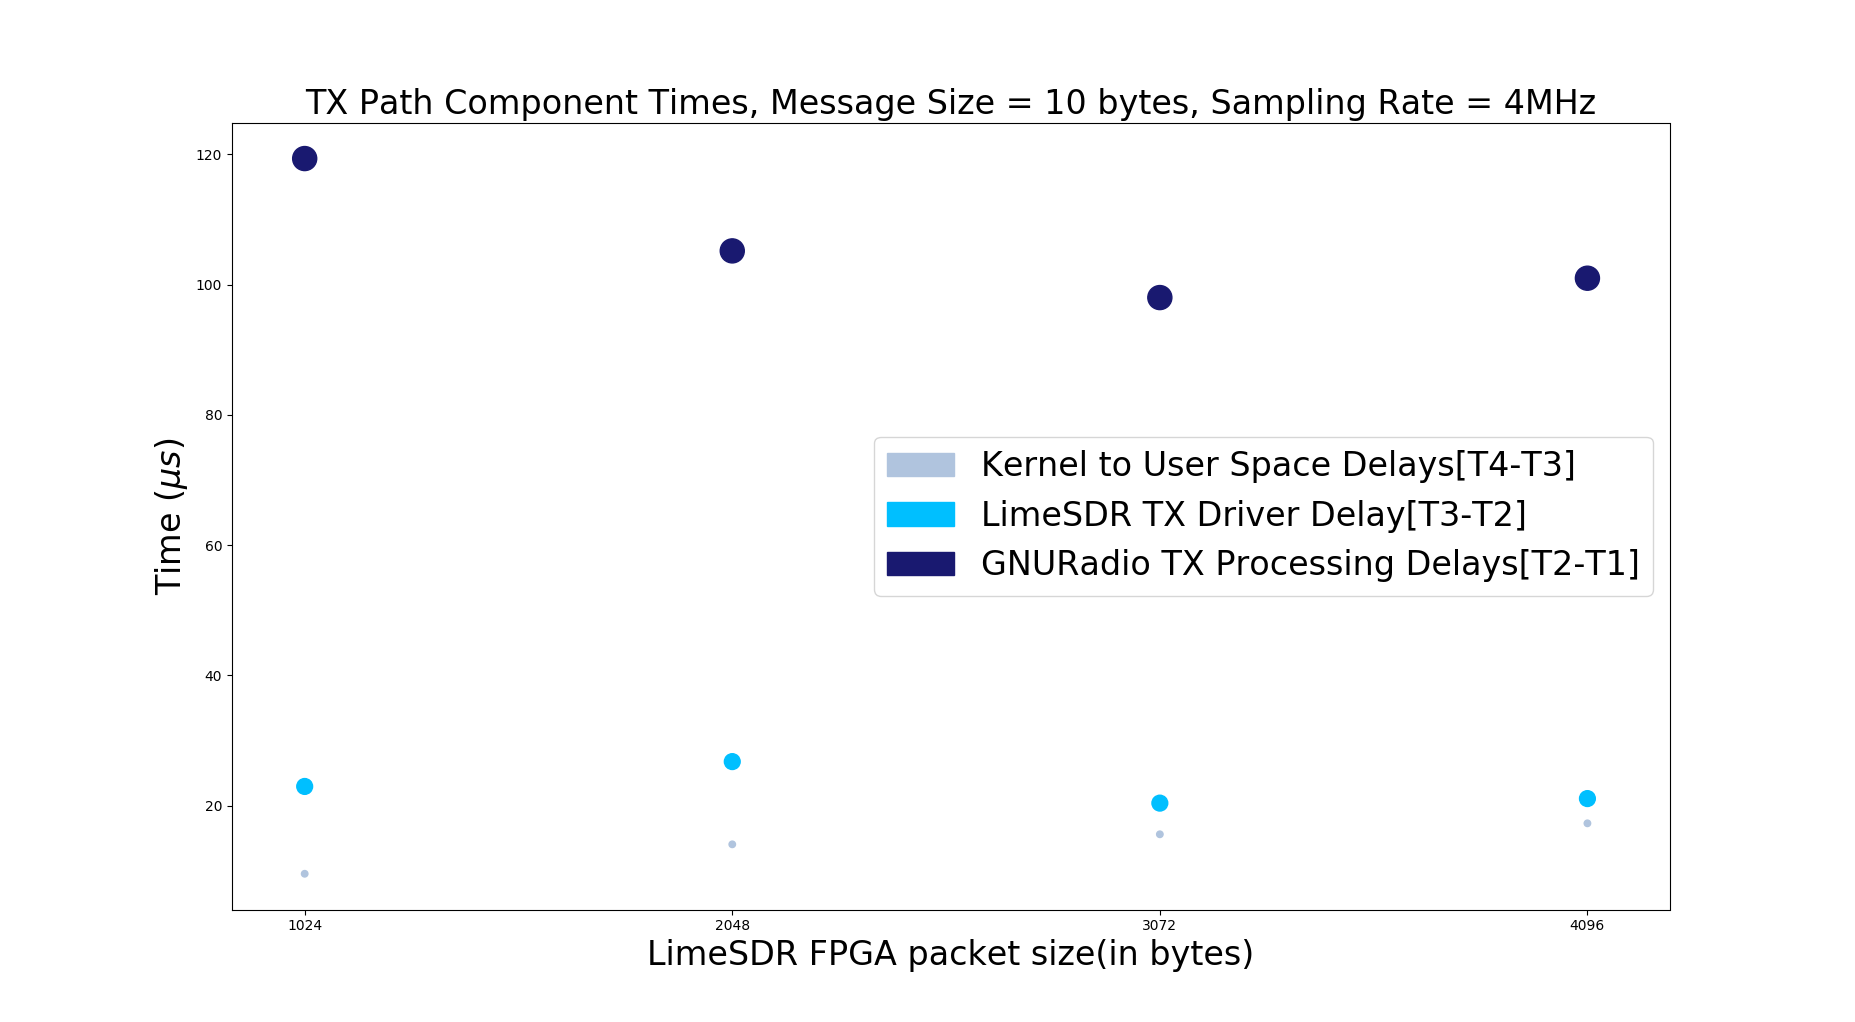
\includegraphics[width=\textwidth]{Thesis/Figure/E4M2-4.png}
\caption{Experiment 4: TX Software Chain Component Delays vs LimeSDR FPGA packet size for the desktop computer (higher processing resources)}
\label{e4_m2_4}
\end{figure}

The TX software delay decreases slightly with increase in the LimeSDR FPGA packet size.
This increase is primarily because of the increase in the GNU Radio TX processing time as shown in Figure \ref{e4_m2_4}.
The GNU radio scheduler needs to schedule the execution of the blocks on the RX flowgraph frequently to handle the lower LimeSDR FPGA packet size.
This cause the scheduler to interleave the processing of the blocks in the TX flowgraph with those in the RX flowgraph, increasing the buffering time for the data in the TX data path.
We think this is the reason for the increase in the GNU Radio TX processing delay.\\

% We see for LimeSDR FPGA packet size of 1024 bytes, we get the highest TX software delay for \texttt{max\_noutput\_items} set to 4000.
% This increase when compared to the results for the \texttt{max n\_output\_value} of 1000 and 2000 can be attributed to the increase of buffering time in the GNU Radio because the blocks now need to process higher number of data elements before handing over to the LimeSDR driver.
% As we are working with muti-core processor, extending one operation longer might make it difficult to pipeline the software processing.\\

\subsection{Influence of processing resources}
\begin{figure}[h!]
\centering
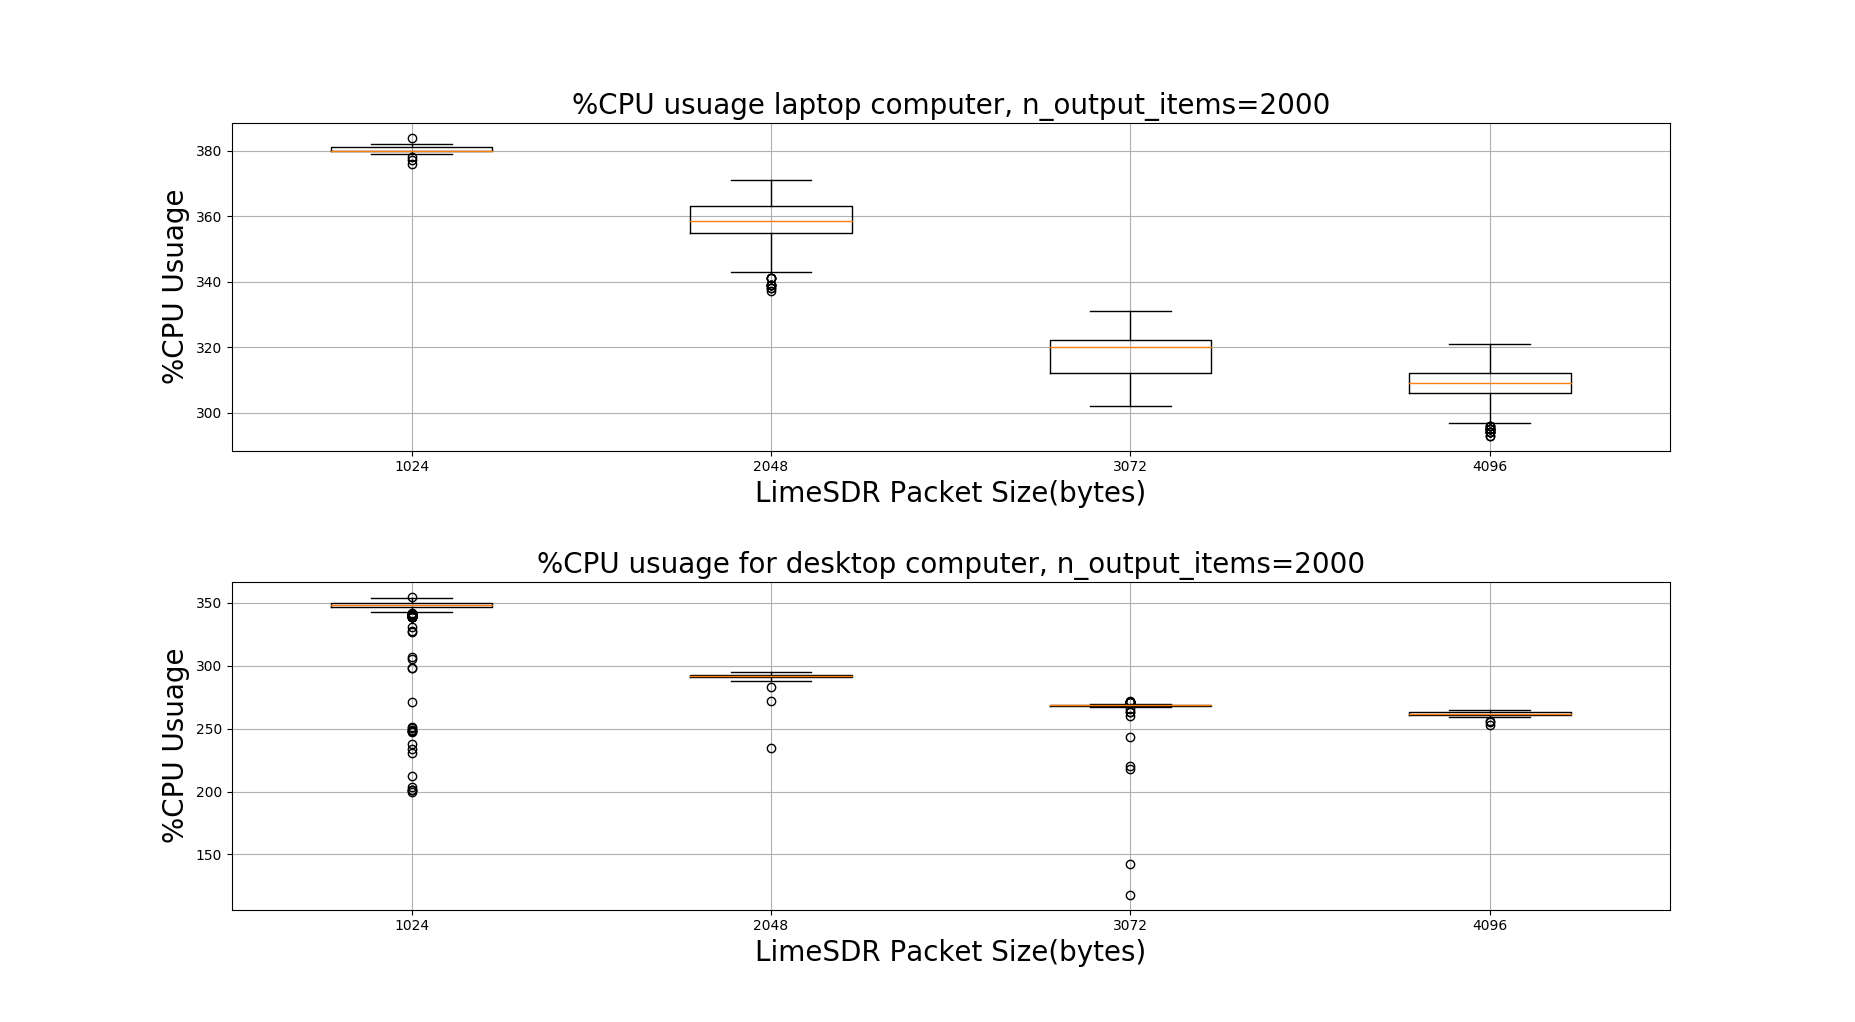
\includegraphics[width=\textwidth]{Thesis/Figure/E4_CPU.png}
\caption{Experiment 4: Comparison of percentage of CPU usage across different LimeSDR FPGA packet sizes for both the host computers}
\label{e4_cpu}
\end{figure}

Figure \ref{e4_cpu} shows the box-plots of the percentage of CPU usuage for the two host computers.
Since both the host computers have four hardware threads, the maximum CPU usage available is 100\% on each of the four threads that is 400 \% CPU usage in total.
The x-axis of the two graphs show the LimeSDR FPGA packet size in bytes, with the y-axis representing the total percentage of CPU usage.
We see that the percentage of CPU usage on the laptop is higher than the desktop computer for all the LimeSDR FPGA packet sizes.
This is mainly because the desktop CPU has higher processing clock speed and two more cores compared to the laptop.
In general the percentage of CPU usage decreases with increase in LimeSDR FPGA Packet size, indicating that lower packet sizes has significant processing overheads. \\
% Also the desktop computer is able to sustain the same performance for the entire duration of the experiments as shown by the very low inter quartile range for the box plots.\\

The laptop has very high CPU usuage for LimeSDR FPGA packet size of 1024 and 2048 bytes. The presence of processing overhead for lower LimeSDR FPGA packet sizes causes the laptop processing resources to throttle as it is already processing at near maximum capacity.
This lack of further processing resources results in increased buffering and unpredictable processing of the flow-graph and that explains the higher mean and standard deviation of the latency for the LimeSDR packet size of 1024 byte and 2048 bytes in Figure \ref{e4_m1_1}.
In case of desktop computer, it operates at close to 350\% for LimeSDR packet size of 1024 bytes, so it still has processing resources available, hence it can continue processing the data packets at the incoming data rate resulting in lower mean and standard deviation of the latency shown in Figure \ref{e4_m2_1}.

\subsection{Effect on throughput}

\begin{figure}[h!]
\centering
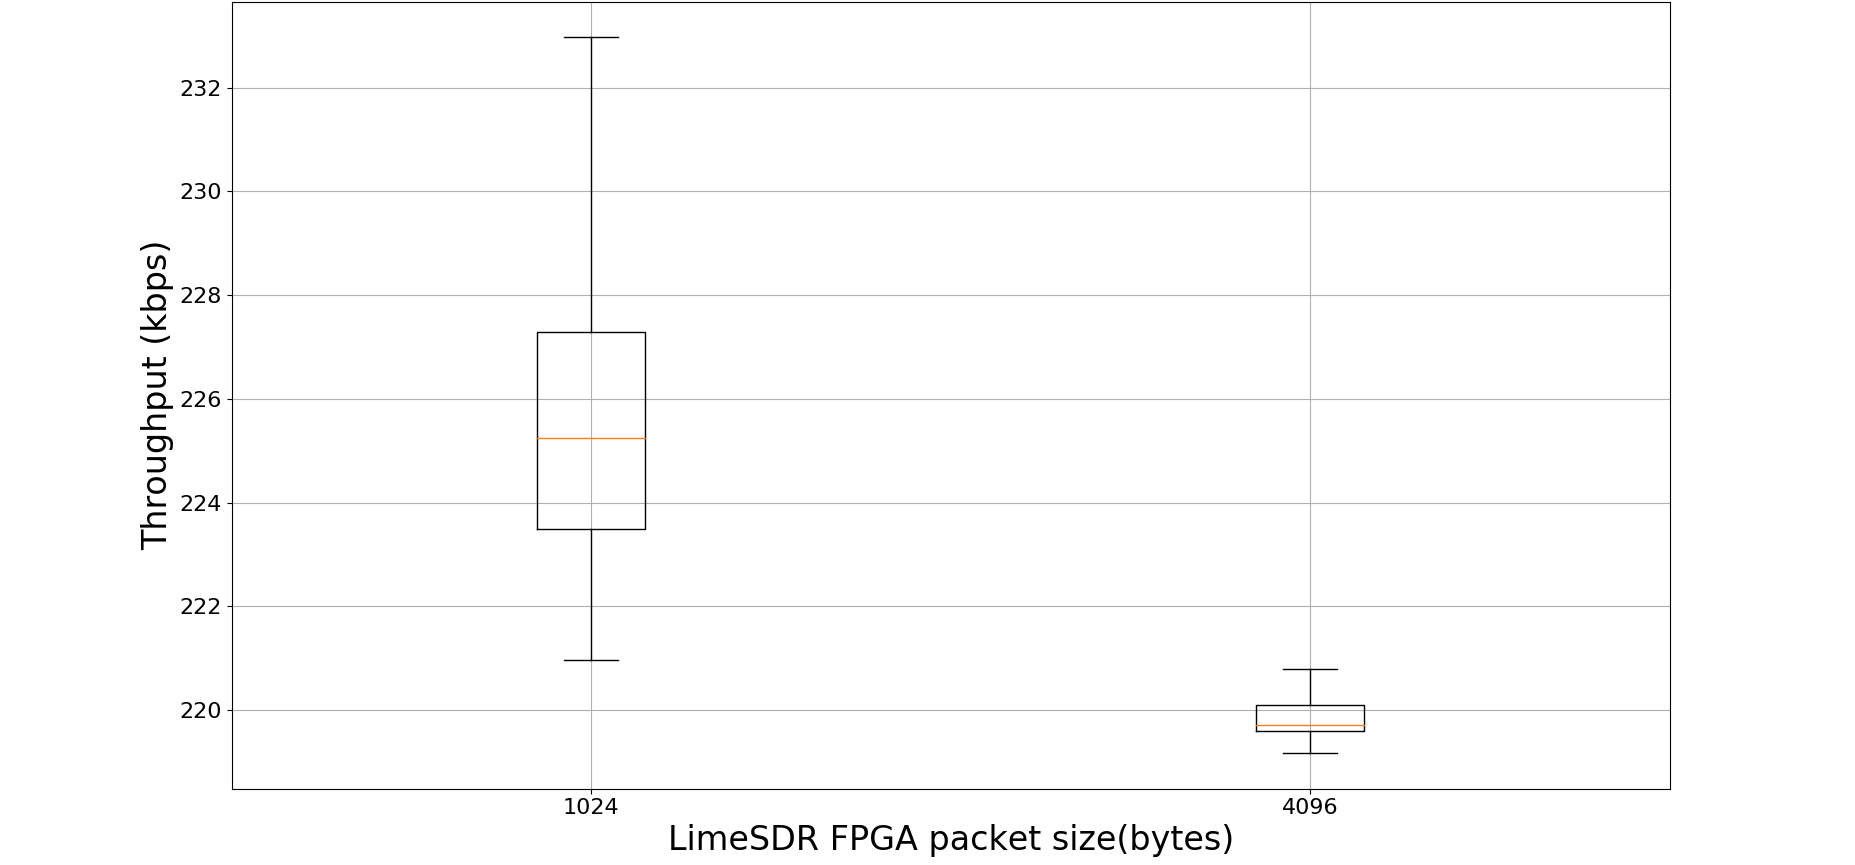
\includegraphics[width=\textwidth]{Thesis/Figure/throughput.png}
\caption{Experiment 4: Comparison of throughput for the best latency case and the default configuration using the desktop computer.}
\label{e4_throughput}
\end{figure}

The results for the  impact of our mitigation strategies on the throughput is presented in Figure \ref{e4_throughput}.
These are presented as box plots of our measured throughput to show the distribution of throughput during the duration of the measurement.
The x-axis shows the LimeSDR FPGA packet size with the y-axis representing the throughput measured using equation \ref{eq:throughput} in kbps.
The LimeSDR packet size of 1024 bytes represents the results for best latency case, while LimeSDR packet size of 4096 bytes shows the results for the default case.
The results highlight that although the variation in throughput is much larger for the best latency case, all the measured throughput values are higher than the one for the default configuration.
The median of the two cases shows a slight increase of approximate 5 kbps from the default case to the best latency case.\\

As the GNU radio blocks process smaller amount of data elements for lower LimeSDR FPGA packet size, multiple execution calls are required which makes the data decoding process dependent on the scheduling mechanism of the GNU radio scheduler. 
So after one execution of the RX flowgraph, if the GNU Radio scheduler schedules the processing of the blocks on the RX flowgraph with higher probability, the data rate will increase.
This is because the LimeSDR provides data at the described sampling rate of 4 Mhz hence the data required for decoding is available.
If the data is consumed faster by repeated calls to the RX flowgraph, the data rate will increase.
Otherwise, if the scheduler schedules the processing of some blocks on the TX Chain or the IEEE 802.15.4 MAC block, the data has to be buffered longer, leading to lower data rate as it increases the the time required ($T_{Complete}- T_{SFD}$) for processing the same amount of data. 
This unpredictability in the scheduling process might explain the high variation of throughput for the best latency case.
On the other hand, with larger USB Transfer size, the number of execution calls decreases making the packet decoder less dependent on scheduling mechanism hence less variance in the throughput for the default case.
The increase in throughput can be attributed to the better pipelined processing with the desktop computer having enough processing resources to handle the overhead of multiple execution calls as explained in the previous subsection.